\section{Anleitung}

Der gegebene Aufbau kann durch spezifische Verkabelung entweder als \hyperref[neben]{\textit{Nebenschlussmaschine}}, oder als \hyperref[reihen]{\textit{Reihenschlussmaschine}} verwendet werden.

Bei Vorhandensein von zwei Spannungsquellen ist auch die Verwendung als \hyperref[fremd]{\textit{fremderregte}} Gleichstrommaschine möglich, dies wird hier jedoch nicht dokumentiert.

\subsection{Nebenschlussschaltung}

Um den Aufbau als Nebenschlussmaschine zu schalten müssen sowohl die Spulen, als auch die Schleifer parallel geschalten werden. (Siehe folgendes Bild)

\begin{figure}[H]
    \centering
    \hfill
    \subfigure[Foto Nebenschlussschaltung]{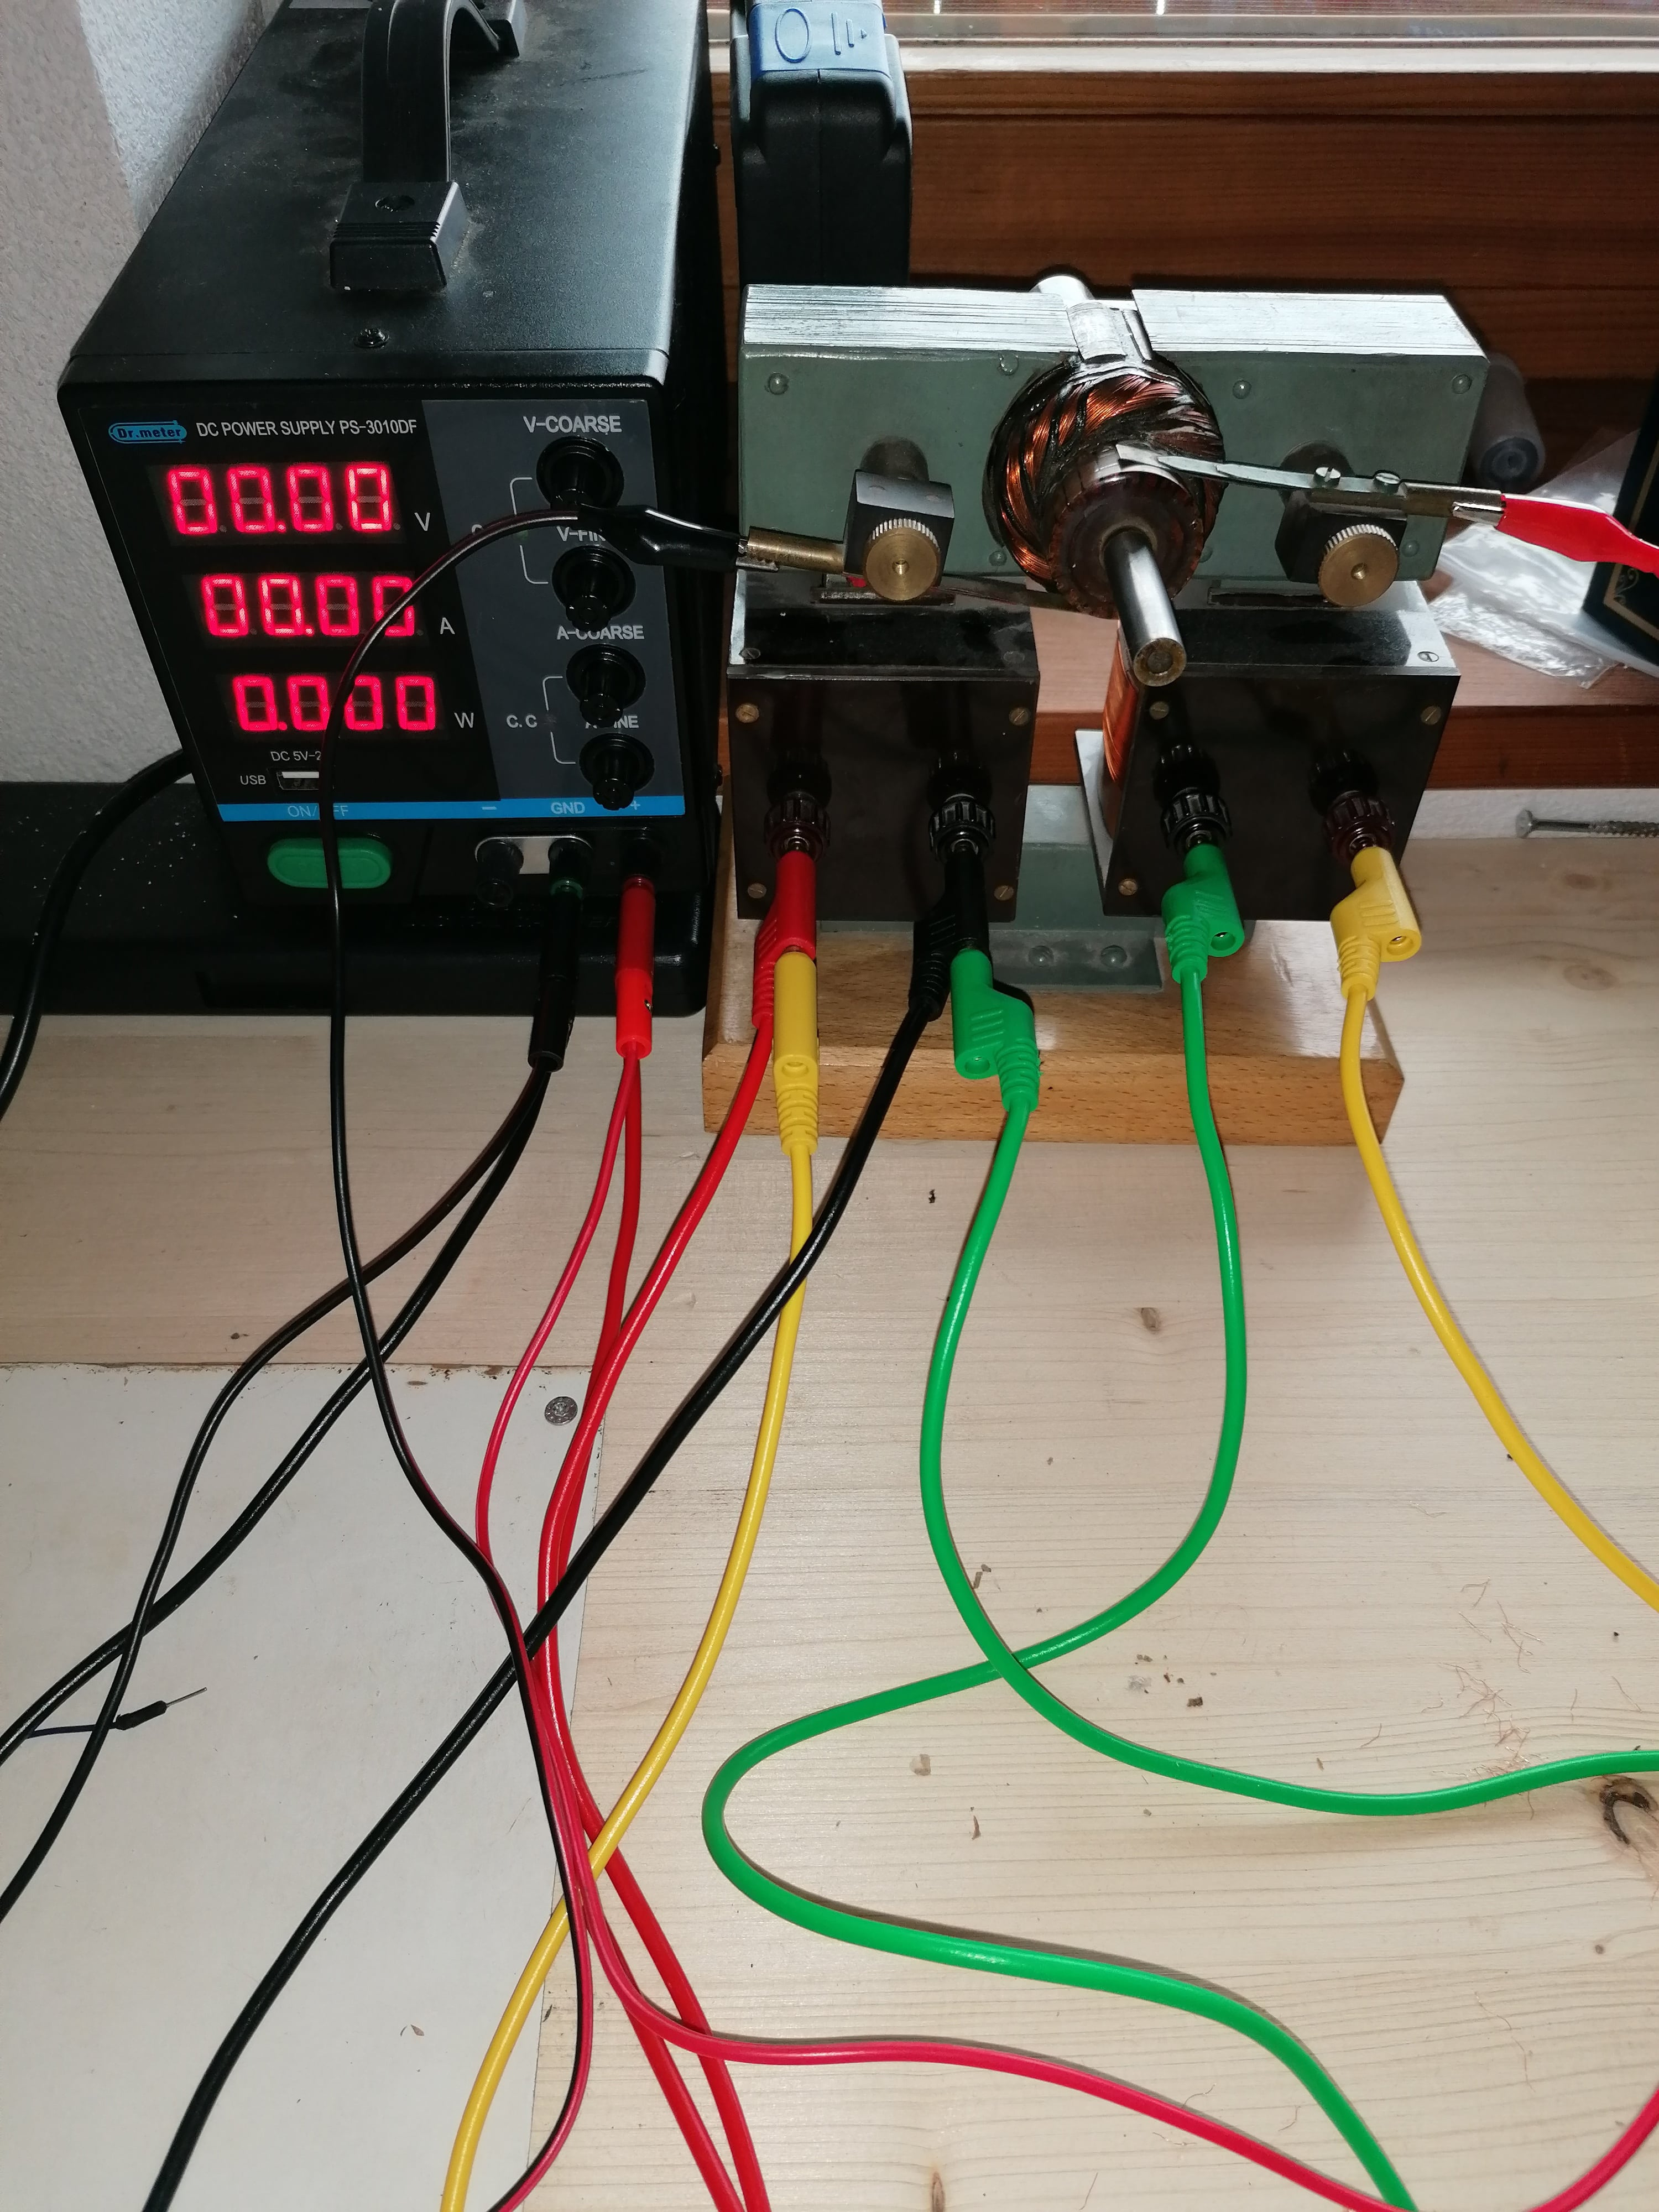
\includegraphics[width=0.3\textwidth]{nebenschluss.jpg}}
    \hfill
    \subfigure[Nebenschlussmaschine laut Wikipedia ~ \cite{wikipedia:neben}]{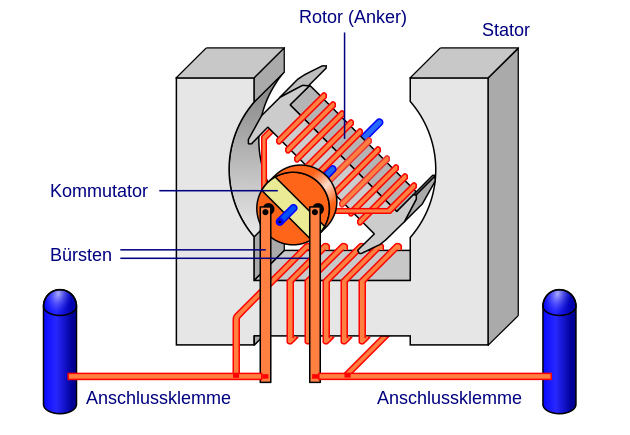
\includegraphics[width=0.3\textwidth]{nebenschlusswiki.png}}
    \hfill
    \caption{Nebenschlussschaltung in 2 Erklärungen}
\end{figure}

Um die Funktionsweise einer Nebenschlussmaschine zu beweisen, können die beiden Verbindungen zu den Schleifern vertauscht werden, was die Drehrichtung umkehrt.

\subsection{Reihenschlussschaltung}

Um den Aufbau als Hauptschlussmaschine zu schalten müssen beide Schaltkreise in Reihe geschalten werden.
Dies bedeutet, dass die Spulen nur über die Schleifer, entweder mit dem positiven oder dem negativen Ausgang der Spannungsquelle verbunden werden dürfen.

\begin{figure}[H]
    \centering
    \hfill
    \subfigure[Foto Reihenschlussschaltung]{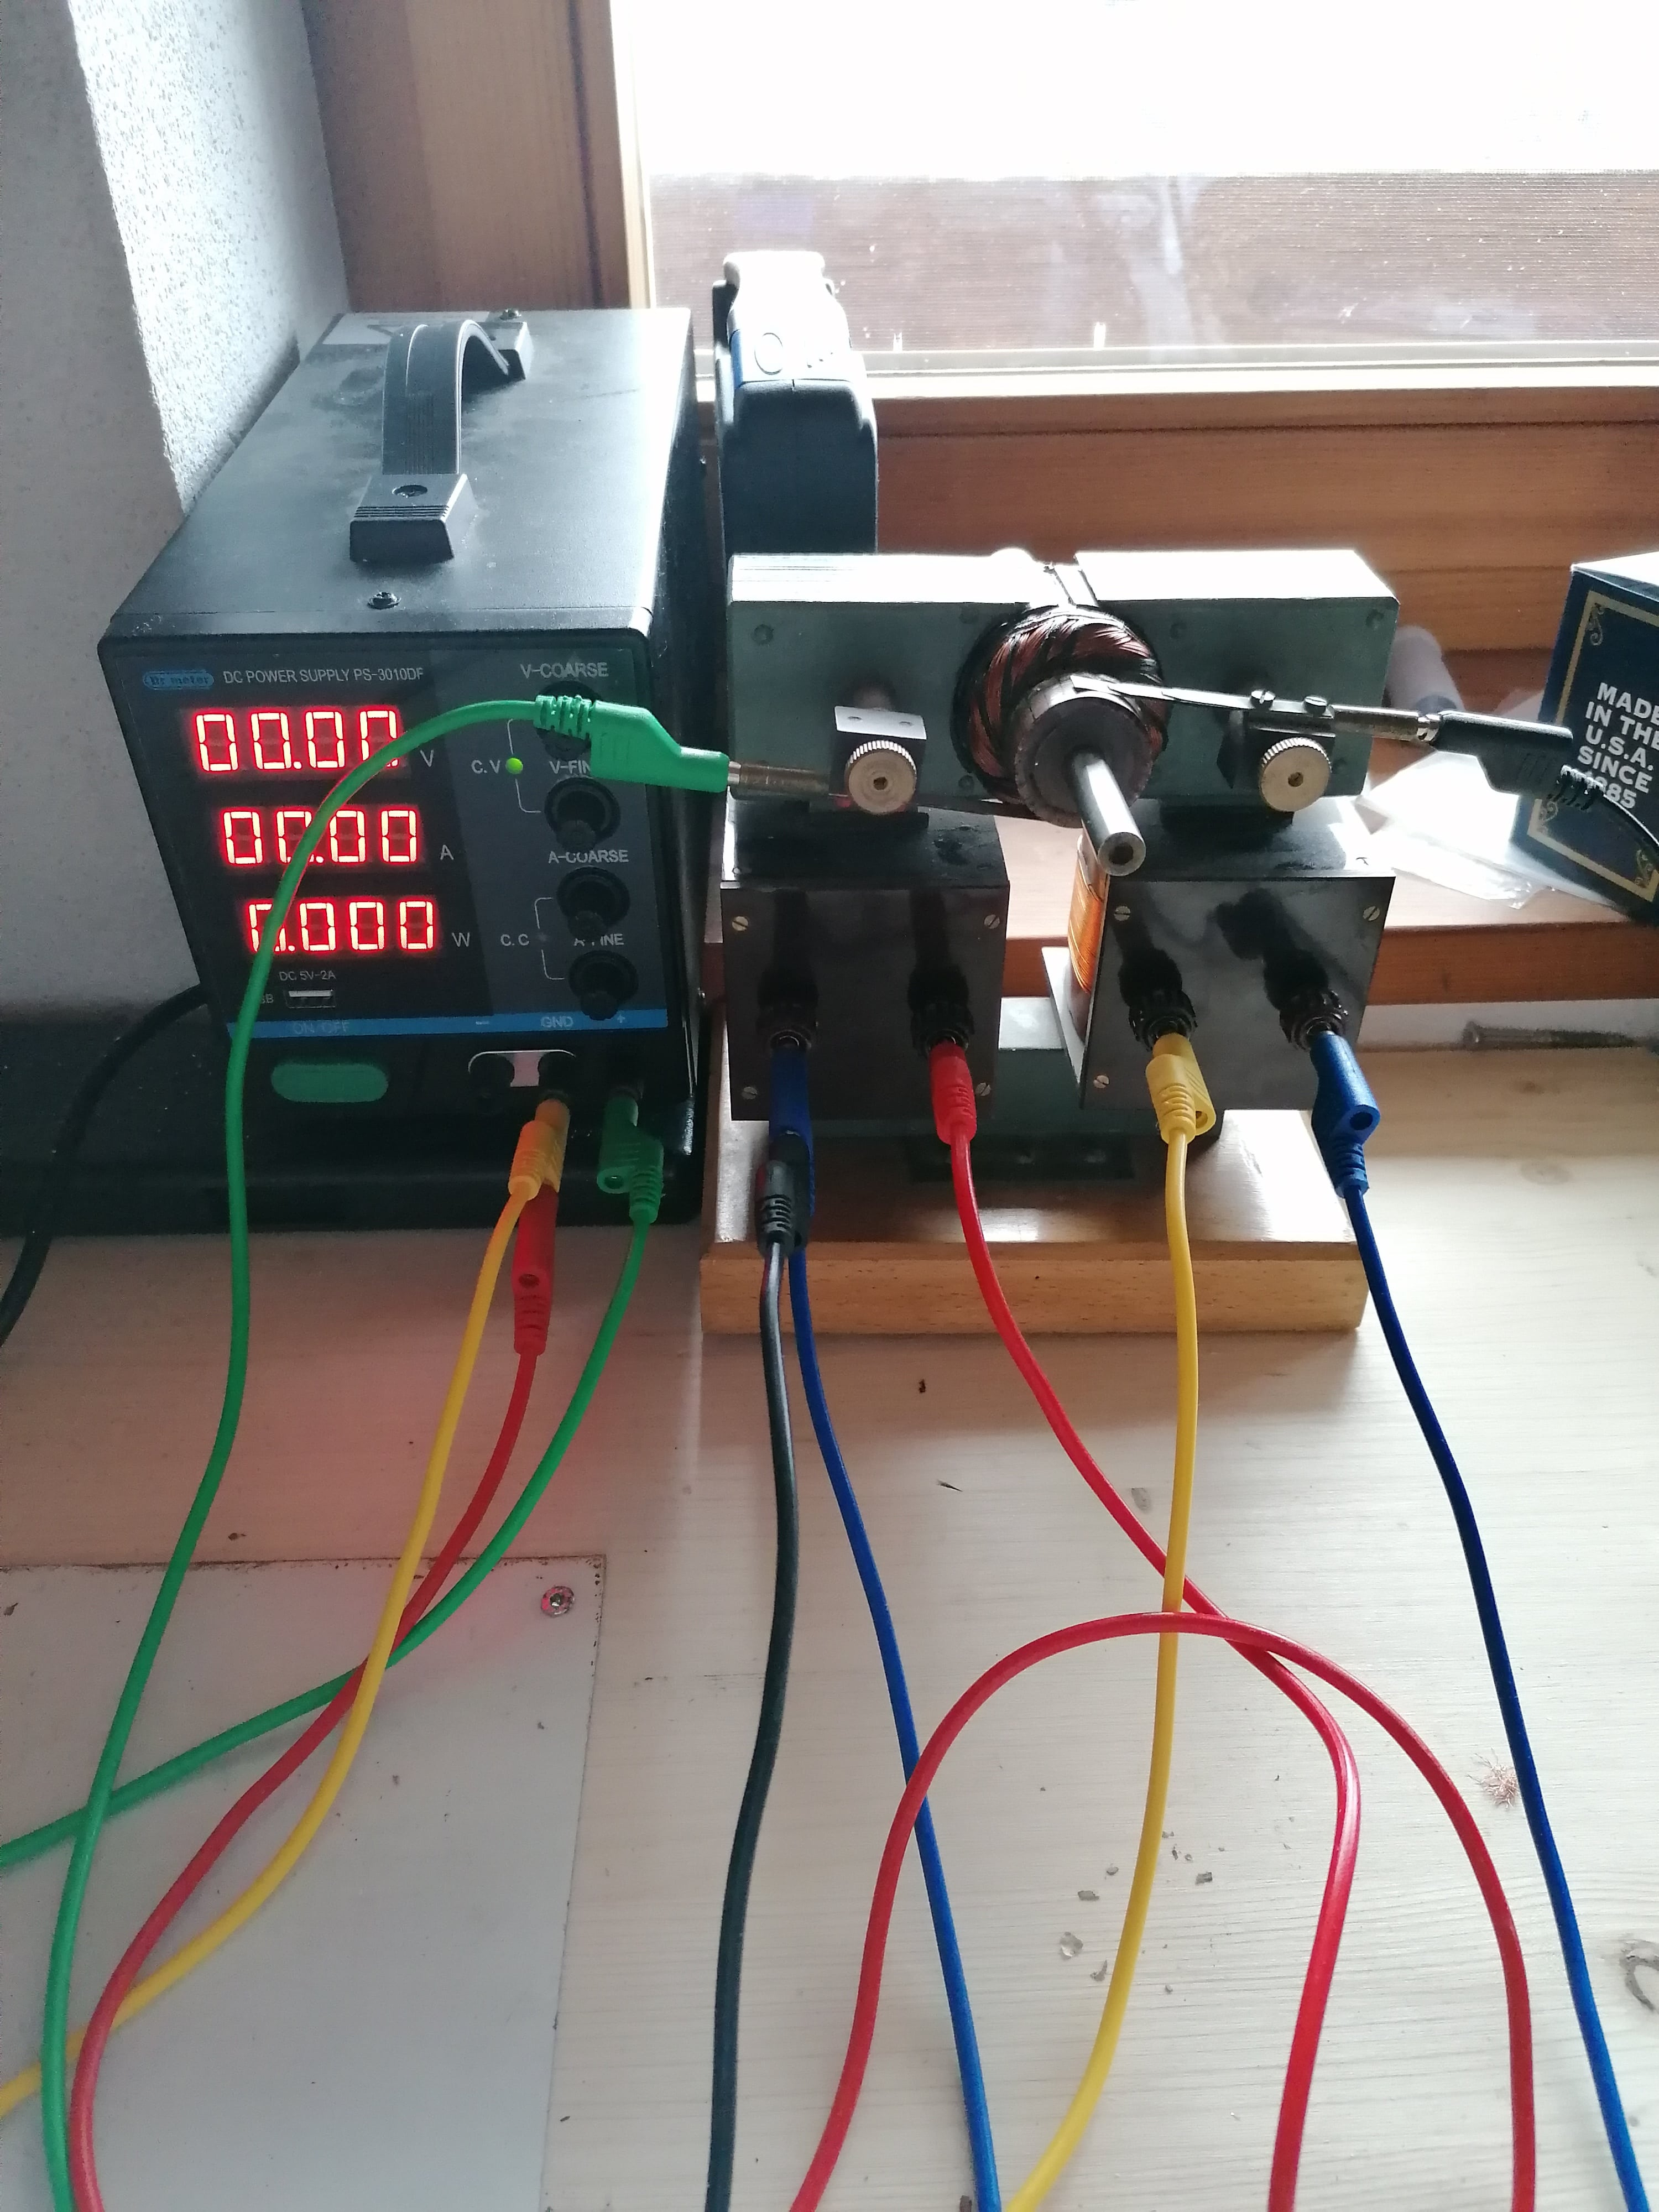
\includegraphics[width=0.3\textwidth]{hauptschluss.jpg}}
    \hfill
    \subfigure[Reihenschlussmaschine laut Wikipedia ~ \cite{wikipedia:reihen}]{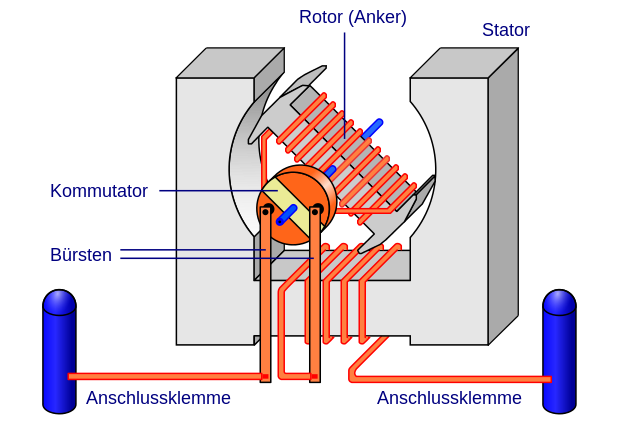
\includegraphics[width=0.3\textwidth]{reihenschlusswiki.png}}
    \hfill
    \caption{Reihenschlussschaltung in 2 Erklärungen}
\end{figure}

Hier kann bewiesen werden, dass bei Vertauschen der Verbindungen zu den Schleifern die Drehrichtung gleich bleibt.